\section{Data}
\label{sec:data}

The calibration problem is defined by two inputs: the household microdata that form the candidate
universe, and the administrative targets the calibrated dataset must reproduce. This section
describes how \populace{} assembles the candidate microdata and how this study selects its targets.
The pipeline is the harness that produces the calibration problem; it is not itself the object of
evaluation.

\subsection{Populace as a construction pipeline}

\populace{} builds a microsimulation dataset by passing a single weighted data structure---a sampling
frame holding the records, their weights, and provenance---through a sequence of stages. Each stage is
a separate package that reads and writes that shared frame: it loads the source surveys, combines them
into one record universe, imputes missing variables, assigns geography, constructs the calibration
targets, and calibrates. Because every stage operates on the same structure, the imputation model and
the calibration method are components that can be swapped without rewriting the pipeline, and the
method studied here is one calibration option among those the pipeline supports.

This modular structure makes the candidate universe a property of the configuration rather than an
accident of the code: the source-loading and imputation stages set what information each record
carries, and calibration sets which records survive and at what weight. \populace{} follows a
generate-then-prune design, assembling the candidate universe once and pruning it to a deployable
budget at the calibration stage.

\begin{figure}[H]
    \centering
    \makebox[\textwidth][c]{%
        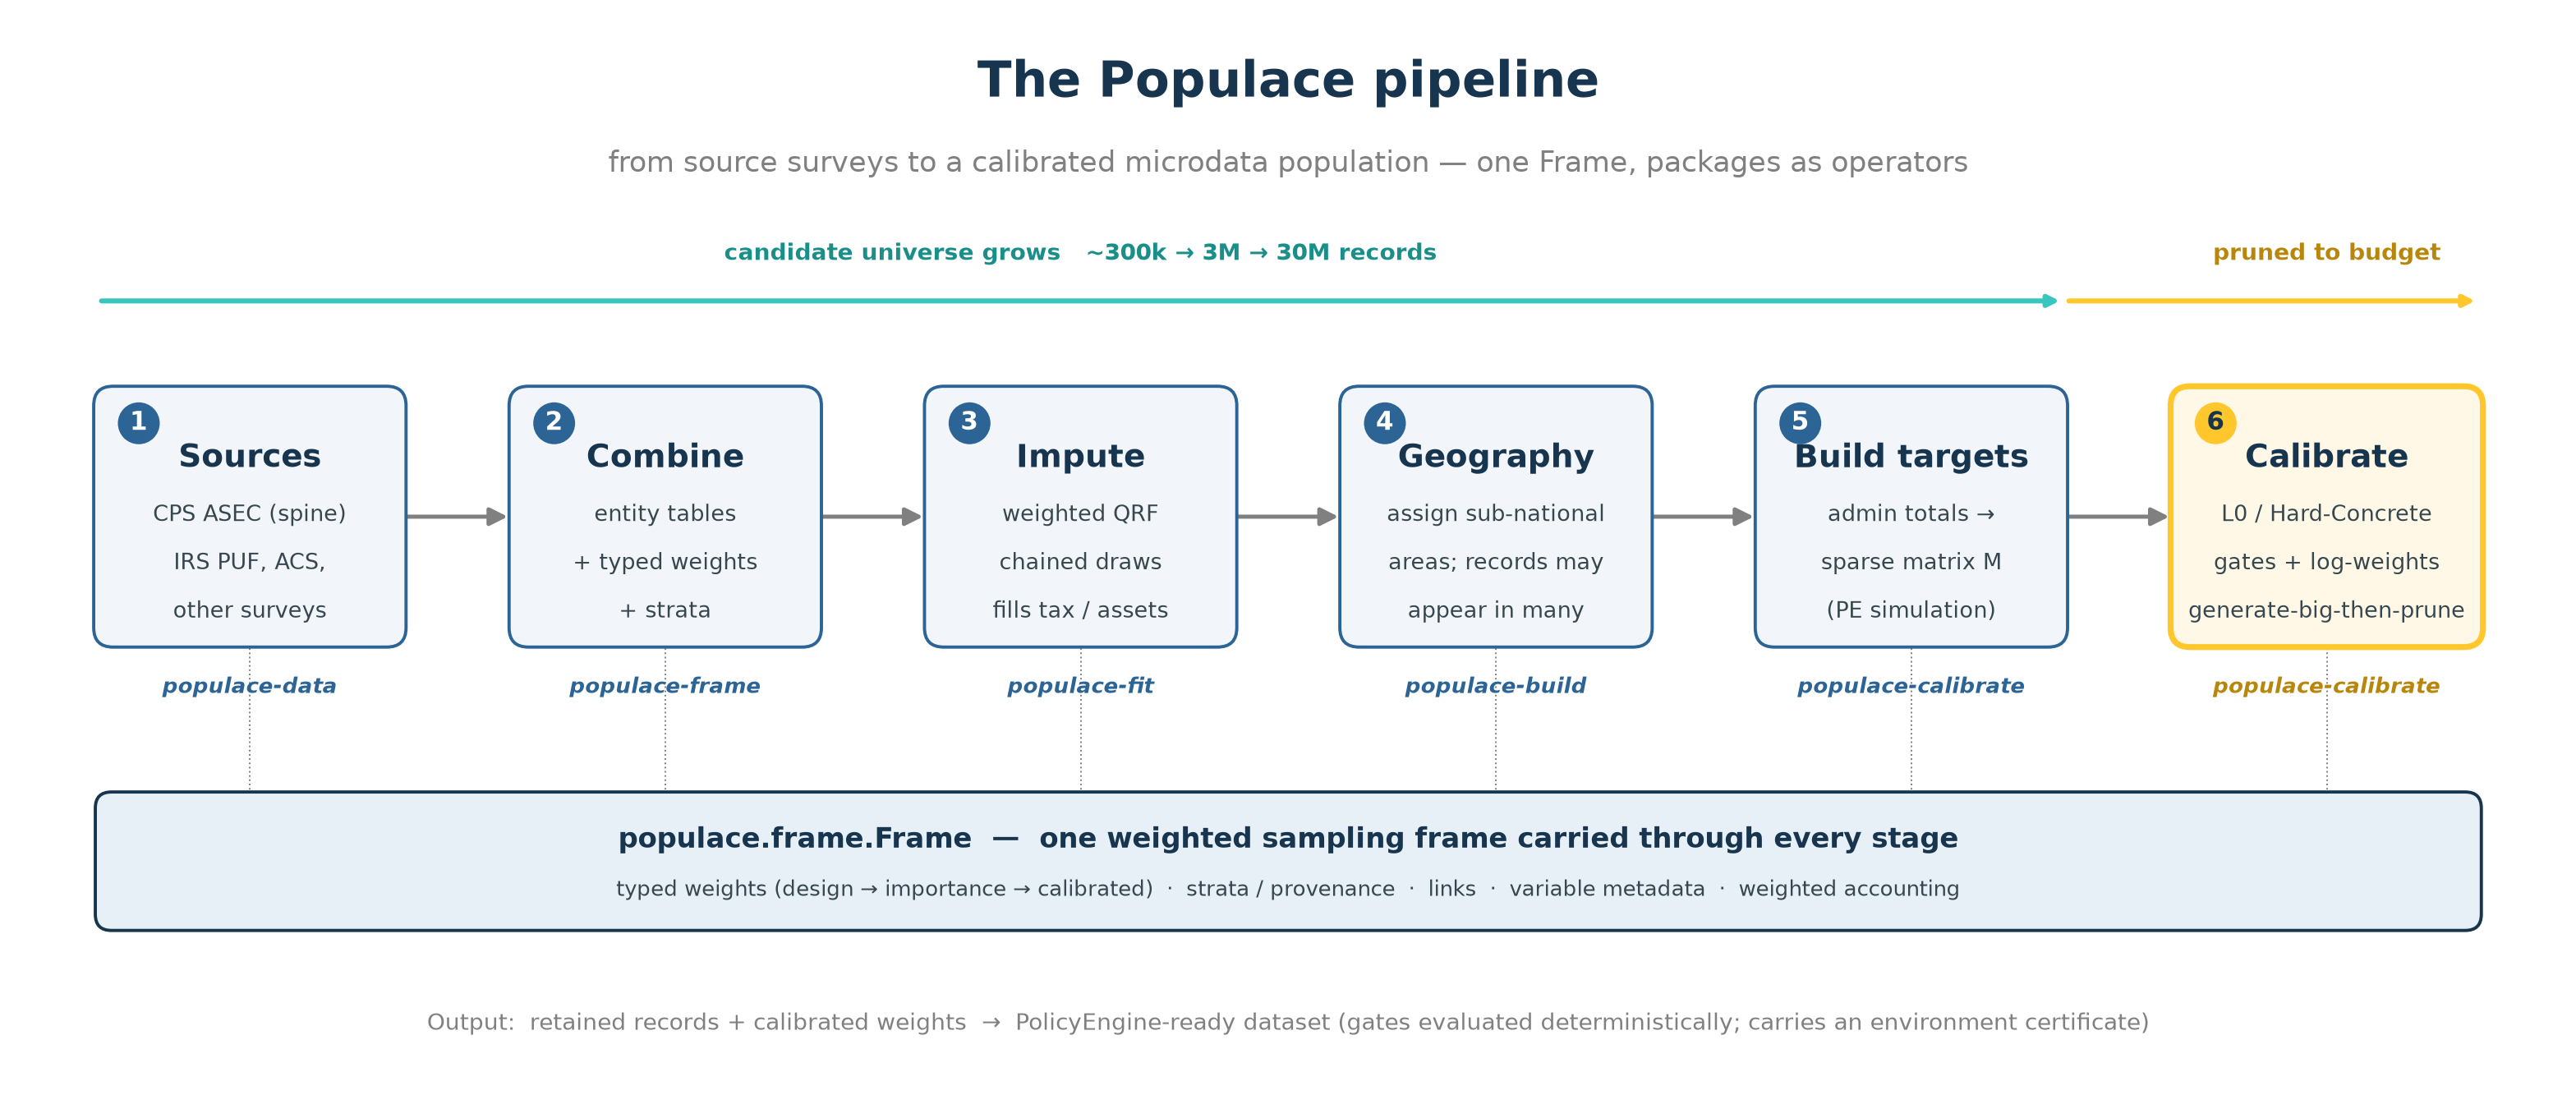
\includegraphics[width=1.18\textwidth]{figures/populace_pipeline}%
    }
    \caption{\populace{} pipeline for the configuration used in this paper: load and combine the
    source surveys, impute missing variables, assign geography, construct the calibration targets,
    and calibrate. The calibration stage is the focus of this paper.}
    \label{fig:pipeline}
\end{figure}

For this build the candidate universe is a three-year pooled ASEC support file for period 2024
(constructed as described below): 337{,}704 household records, one row per candidate household placement.
We pin the exact build for
reproducibility: \populace{} commit \texttt{558e46c1}, base H5 SHA-256 beginning
\texttt{ec290055}, Ledger facts SHA-256 beginning \texttt{82cd9e87}, and target-registry version
\texttt{5a22295b02b6}. The run resets household weights to a uniform prior before calibration, so the
comparison is about support selection and reweighting rather than inherited survey weights.

\subsection{Base microdata}

\subsubsection{Current Population Survey}

The primary source is the Current Population Survey Annual Social and Economic Supplement
\citep[CPS ASEC;][]{census2024}, a nationally representative household survey from the US Census
Bureau and the Bureau of Labor Statistics. The CPS provides demographic structure, household
relationships, labour income, transfer income, and reported participation in programmes such as
SNAP, Medicaid, SSI, and TANF.

The candidate universe is not a single survey year. To widen the support before pruning, \populace{}
pools the three most recently published CPS ASEC files---one per survey year---and ages the two earlier
vintages forward to the latest year, so all three are expressed at a common period, 2024 for this build.
Pooling three years rather than one substantially increases the number of candidate records and widens the
variation the frame carries, while aging keeps the older vintages comparable to the most recent one; the result is a
larger, richer candidate frame that still inherits the CPS survey design. This is the generate side of the
generate-then-prune setting: the pooled file is deliberately larger than the deployable dataset, and
calibration decides which of its 337{,}704 records survive.

The CPS is not a complete tax-benefit dataset on its own. Some tax variables are missing, others are
measured with error, and top incomes are imperfectly captured relative to tax records
\citep{burkhauser2012}. Benefit receipt is also underreported relative to administrative sources
\citep{meyer2015}. The pipeline therefore augments the CPS before calibration.

\subsubsection{Imputation from administrative and survey sources}

The pipeline enriches the CPS base by imputing variables from administrative and survey donors. It
imputes tax-return detail from the IRS Public Use File \citep[PUF;][]{bryant2023a} onto CPS records
following \citet{woodruff2024}: the PUF carries detailed tax-return information but lacks household
structure and demographic coverage, so quantile regression forests \citep{meinshausen2006quantile}
predict the PUF variables on the CPS; \citet{meyer2021} assess the accuracy of such
survey--administrative tax imputations. The imputation is sequential and regime-gated, drawing from a
weighted bootstrap, so later variables condition on earlier imputed values. The same machinery draws
further variables from the donors in Table~\ref{tab:donors} where the CPS is thin. Each step adds
variables to the existing households rather than new records, so the candidate universe stays at one
row per household.

\begin{table}[H]
\centering
{\tablefont
\begin{tabular}{@{}p{0.30\textwidth}p{0.60\textwidth}@{}}
\toprule
Donor source & Variables contributed (this build) \\
\midrule
CPS ASEC & Household and person structure, demographics, labour and transfer income, programme participation, unit assignment \\
IRS PUF (2015, uprated) & Itemized-deduction detail, QBI/SSTB components, partnership and S-corp income, selected tax detail \\
CPS ORG & Hourly wage, paid-hourly and union status, weekly hours, overtime inputs \\
SCF & Wealth and net-worth components \\
SIPP & Tips \\
MEPS-IC & Employer-sponsored insurance premiums \\
ACS (2022) & Rent (pre-subsidy) \\
CMS marketplace PUFs and CPS ASEC & ACA take-up and the benchmark-plan ratio \\
\bottomrule
\end{tabular}
}
\caption{Donor sources imputed onto the CPS base for this build, from the \populace{}-US release stage
manifest. The stages run in a fixed order, each conditioning on the variables already imputed.}
\label{tab:donors}
\end{table}

\subsubsection{Geography}

Each household carries a geographic identity. The CPS ASEC reports the household's state, and
\populace{} attaches congressional-district identifiers so the same frame can be calibrated against
national, state, and district targets. The current support file intentionally contains many more
candidate household placements than the final deployable file should retain. That is the build-big,
then-prune setting: \populace{} creates a support rich enough to cover the target surface, and the
calibration method decides which records survive.

\subsection{Calibration targets}

The target system combines aggregates from several administrative sources at the national, state, and
congressional-district levels. The headline experiment uses the full materialized target surface compiled
from the current \populace{} US fiscal registry: 37{,}053 Ledger facts produce 32{,}633 targets after
materialization against the candidate frame. Appendix~\ref{app:targets} lists the target families and
sources. The exact counts come from the run registry rather than from a pipeline-wide inventory.

\begin{table}[H]
\centering
{\tablefont
\begin{tabular}{@{}p{0.52\textwidth}l r@{}}
\toprule
Target family & Geographic level & Targets \\
\midrule
IRS Statistics of Income (\texttt{irs\_soi}) & National, state, district & 30{,}252 \\
Census population estimates (\texttt{census\_population}) & National, state & 936 \\
Medicaid and CHIP, CMS (\texttt{cms\_medicaid}) & National, state & 102 \\
ACA marketplace, CMS (\texttt{cms\_aca}) & State & 102 \\
SNAP, USDA (\texttt{usda\_snap}) & National, state & 52 \\
State income tax, Census STC (\texttt{state\_income\_tax}) & State & 44 \\
TANF, HHS ACF (\texttt{hhs\_acf\_tanf}) & National, state & 30 \\
Social Security OASDI, SSA (\texttt{ssa}) & National & 6 \\
JCT tax expenditures (\texttt{jct}) & National & 5 \\
CBO revenue projections (\texttt{cbo}) & National & 4 \\
Medicare, CMS (\texttt{cms\_medicare}) & National & 1 \\
\midrule
\textbf{Total} & & \textbf{31{,}534} \\
\bottomrule
\end{tabular}
}
\caption{Full materialized Populace target surface used in this study, by family and geographic level.
The surface contains 23{,}450 congressional-district targets, 7{,}615 state targets, and 469 national
targets.}
\label{tab:target_subset}
\tablenote{Counts are read from the full-surface run registry. In the headline experiment all targets,
including \texttt{cbo}, are fit and scored; holdout variants are supplemental diagnostics
(Section~\ref{sec:oos}). The source for each family is listed in Appendix~\ref{app:targets}.}
\end{table}

